\chapter{方程的数值解}
不管白猫黑猫,能捉到老鼠的就是好猫\\
\makebox{}\hfill——邓小平

\section*{学习目标}
\begin{todolist}
 \item 了解解析解和\gls{numsolution}的区别
 \item 通过图像或者多项式的符号变化大致判断根的范围
 \item 了解二分法的思想
 \item 理解级数收敛的极限可以用于预估方程的解
 \item 通过简单的迭代$x_{n+1} = f(x_n)$求算指定精度的方程数值解
\end{todolist}
\clearpage

\section{高次多项式的根}
二次方程$ax^2+bx+c=0$存在解析解$x=\frac{-b\pm \sqrt{b^2-4ac}}{2a}$。但是一旦涉及到更高次的方程之后,配方或者其他的代数思路就没用了,所以当时的人们暂时没有想出解决三次方程的方法\footnote{1500-1515年,费罗找出了$x^3+px=q$,这样的三次方程的代数解法,记载于卡尔达诺的书本上,采用的例子是$x^3+6x=20$}。没有解析解,不代表某个特定的方程是求不出其数值解的。

\subsection*{图像法}
在IGCSE阶段我们就学习过图像的交点就是方程的解。例如下图
\begin{figure}[H]
\centering
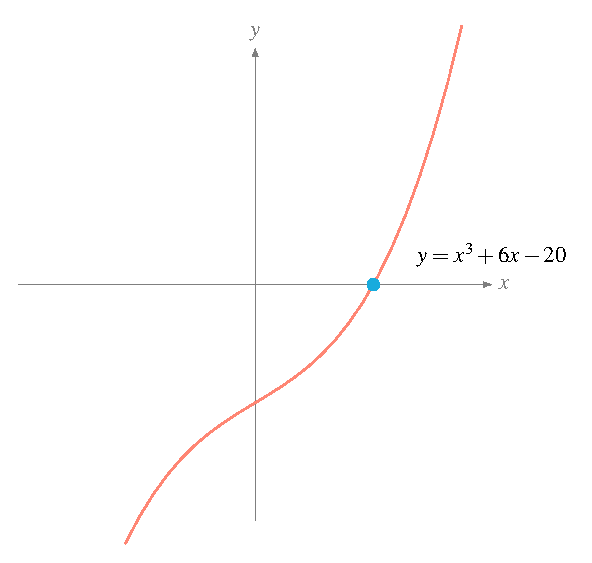
\includegraphics[width=0.8\textwidth]{polysolution}
\caption{多项式函数和$x$轴的交点,就是对应方程的解}
\end{figure}
但是,非常缺憾的是,我们手工绘制的图像并不是非常精确的,因此得到的结果只能算作是一种\emph{预估}。那么怎么样才能让这个预估更加的精确一点?

\subsection*{变号与二分法逼近}
针对于任意连续函数,\gls{jiezhi}始终成立:
\begin{theorem}
The Intermediate Value Theorem states that if $f$ is a \emph{CONTINOUS} function whose domain contains the interval $[a, b]$, then it takes on any given value between $f(a)$ and $f(b)$ at some point within the interval.
\end{theorem}

那么当两个端点值分别为一正一负的情况时,介值定理就变成了\gls{bolzano},其定义如下:
\begin{theorem}
If a function is \emph{CONTINOUS} in the closed interval $[a,b]$ and $f(a)\cdot f(b)<0$. There should be at least one zero point in the interval.
\end{theorem}
因此,该解必定是在$[a,b]$之间的某个数

\begin{ExampleBox}
The equation $x^5-3x^3+x^2-4=0$ has one positive root. Verify by calculation that this root lies between $1$ and $2$.\\
\makebox{}\hfill Adapted from 2016 spring qp32 Q3
\tcblower
因为$1^5-3\times 1^3+1^2-4=-5$,$2^5-3\times 2^3+2^2-4=8$。两个端点值一正一负。因此正数解必定在$1$和$2$之间
\end{ExampleBox}
\clearpage


\section{迭代法}
\subsection*{二分法(了解)}
知道根所在的范围并不足够,于是,我们有一种暴力破解求算的方法——\gls{dichotomy}。既然博尔扎诺定理在连续函数上都能继续使用,那么我们便只要埋头缩小根的区间即可。因此该方法就是纯粹进行运算的暴力破解方法。
\begin{ExampleBox}
利用二分法缩小$x^5-3x^3+x^2-4=0$的根的区间
\tcblower
已知该正数解在$[1,2]$之间,利用二分法,该区间的中间点是$\frac{1+2}{2}=1.5$。检验$f(1.5)=-4.28125$。因此,可以缩小该区间到$[1.5,2]$之间;

然后重复该步骤,检验下一个中间值$f(1.75)=-\frac{617}{1024}$。因此再次缩小区间到$[1.75,2]$之间;如此循环下去
\end{ExampleBox}
\clearpage

\subsection*{数列迭代收敛}
\noindent\begin{minipage}{0.5\linewidth}
该方法的是考试的重点,核心原理是使一个数列$x_1,x_2,x_3,\ldots,x_n,x_{n+1}\ldots$\gls{converge}。并且后一项可以看成是前一项的函数$x_{n+1}=f(x_n)$。因此如果该数列的数值最后收敛于$L$的话,那么必定存在$L=f(L)$,该表达式能够使原方程成立。所以,最后要做的事情就是利用计算器的$ans$功能逼近该极限$L$。

重复执行一系列运算步骤,从前面的量依次求出后面的量的过程。这种思维方法叫做\gls{iteration}
\end{minipage}
\hfill
\begin{minipage}{0.3\linewidth}
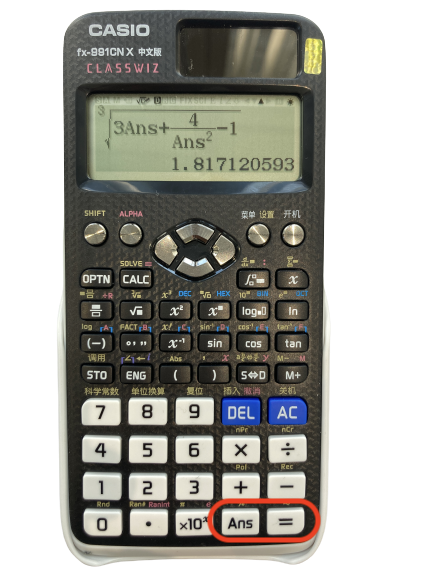
\includegraphics[width=\textwidth]{casio}
\captionof{figure}{利用ans键}
\end{minipage}

\begin{ExampleBox}
The equation $x^5-3x^3+x^2-4=0$ has one positive root.\\
a). Prove That the equation can be arranged in the form:
\[
	x=\sqrt[3]{\left(3x+\frac{4}{x^2}-1\right)}
\]

b). Use an iterative formula based on this rearrangement to determine the postive root correct to 2 decimal places. Give the result of each iteration to 4 decimal places.\\
\makebox{}\hfill Adapted from 2016 spring qp32 Q3
\tcblower
a). 略

b). 因此采用迭代的方法的话,数列$\{x_n\}$必定满足如下的关系:
\[
	x_{n+1} =\sqrt[3]{\left(3x_n+\frac{4}{x_n^2}-1\right)}
\] 
而且,该数列$\{x_n\}$最后收敛的值$L$是方程的解。由于题目已知条件,该值$L$必定介于$[1,2]$之间,因此$x_1=1$或者$x_1=2$都可以,甚至为了减少计算次数,选择$[1,2]$区间上的任何数值,都能最后收敛于$L$。在这里选用$x_1=2$产生如下表格:
\begin{table}[H]
\centering
\begin{tabular}{l|c|c|}
\hline
\multicolumn{1}{|l|}{$x_1=2.0000$} & $x_{n+1} =\sqrt[3]{\left(3x_n+\frac{4}{x_n^2}-1\right)}$ & Converge to 2 d.p.? \\ \hline
                                   & $x_2=1.81712$                                            & No                  \\ \cline{2-3} 
                                   & $x_3=1.78242$                                            &                     \\ \cline{2-3} 
                                   & $x_4=1.77647$                                            &                     \\ \cline{2-3} 
                                   & $x_5=1.77548$                                            &                     \\ \cline{2-3} 
                                   & $x_6=1.77532$                                            & Yes                 \\ \cline{2-3} 
\end{tabular}%
\end{table}
从后面$x_5$可以看出该极限在$1.775$左右,因此如果保留到小数点后两位的话,可以把$1.78$作为该方程的解。
\end{ExampleBox}
以上这两种方法就是通过极限的思想,并不能直接求算方程的解,但是

\begin{TaskBox}
1. 如果从$1$开始,每次迭代的结果是什么?\\
2. 表格上从第几项开始就可以认为数据近似稳定了?\\
3. 图片上有一个小彩蛋。
\end{TaskBox}
\clearpage


\begin{SummBox}
1. 对于任何方程,如果是连续的,那么可以根据介值定理或者博尔扎诺定理确定方程的根所处的区间。要求是$f(a)\cdot f(b)<0$,在该区间的端点值发生了符号改变\\

2. 迭代法逼近数值解的过程是:
\begin{itemize}
	\item 重新排列表达式,将$f(x)=0$ 改写为 $x=g(x)$的形式;
	\item 将等价的函数当成是\textbf{数列}处理,改写为$x_{n+1}=g(x_n)$;
	\item 选择$f(x)=0$的根所在区间内的端点值(也可以是任意值)带入到数列表达式中,利用计算器的ans功能进行迭代
	\item 如果最后数据值趋于稳定,满足要求,则迭代结束;如果迭代之后结果波动非常剧烈,则是因为数列的表达式选择错误,需要从第一步开始重新调整表达式
\end{itemize}

\end{SummBox}



